\documentclass[12pt]{article}

\usepackage[left=25mm, top=20mm, right=15mm, bottom=20mm, nohead, foot=10mm]{geometry} 
\usepackage{tikz}
\usepackage[simplified]{pgf-umlcd}

\begin{document}
	In class-based programming, the factory method pattern is a creational pattern that uses factory methods to deal with the problem of creating objects without having to specify the exact class of the object that will be created. 
	
	\vspace{10 mm}
	
	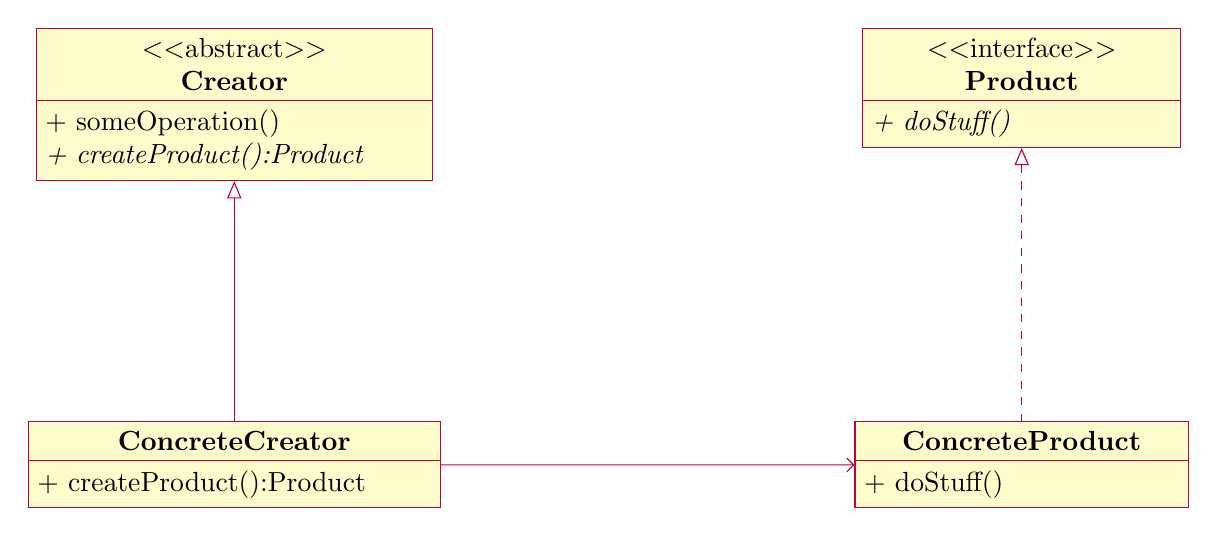
\begin{tikzpicture}
		\begin{abstractclass}[text width=4.8cm]{Creator}{0 ,0}
			%\attribute{name:attribute type}			
			%\attribute{name:attribute type = default value}
			\operation{+ someOperation()}
			\operation[0]{+ createProduct():Product}
		\end{abstractclass}
	
		\begin{class}[text width=5cm]{ConcreteCreator}{0 ,-5}
			\inherit{Creator}
			%\attribute{name:attribute type}			
			%\attribute{name:attribute type = default value}
			\operation{+ createProduct():Product}
		\end{class}
		
		\begin{interface}[text width=3.8cm]{Product}{10, 0}
			%\attribute{name:attribute type}			
			%\attribute{name:attribute type = default value}
			\operation[0]{+ doStuff()}
		\end{interface}
	
		\begin{class}[text width=4cm]{ConcreteProduct}{10, -5}
			\implement{Product}
			%\attribute{name:attribute type}			
			%\attribute{name:attribute type = default value}
			\operation{+ doStuff()}
		\end{class}
		
		\unidirectionalAssociation{ConcreteCreator}{ }{ }{ConcreteProduct}
		
	\end{tikzpicture}
\end{document}

